\documentclass{article}

%===============================================================================
%
%===============================================================================
\usepackage[english]{babel}
\usepackage[T1]{fontenc}
\usepackage[utf8]{inputenc}
\usepackage{float}
\usepackage{graphicx}
\usepackage{multicol}
\usepackage{caption}
\usepackage{subcaption}
\usepackage{vmargin}
\usepackage[colorlinks]{hyperref}
\usepackage{indentfirst}
\usepackage{wrapfig}
\usepackage{dirtytalk}
\usepackage[newfloat]{minted}
\usepackage{cleveref}

\graphicspath{{img/}}

% Možnost referencí na footnotes https://tex.stackexchange.com/a/35044/160241
\makeatletter
\newcommand\footnoteref[1]{\protected@xdef\@thefnmark{\ref{#1}}\@footnotemark}
\makeatother

%===============================================================================
%
%===============================================================================
\title{Quadtree Spatial Partitioning for Unity}
\author{Daniel Dolejška\\\small\texttt{dolejskad@gmail.com}\\\small\url{https://github.com/dolejska-daniel/unity-quadtree}}
\date{\today}

%===============================================================================
%
%===============================================================================
\begin{document}

%-----------------------------------------------------------
%   Title page
%-----------------------------------------------------------
\maketitle

\tableofcontents

\newpage

%-----------------------------------------------------------
%   Package introduction & contents
%-----------------------------------------------------------
\section{Introduction}
This package provides generic implementation of the quadtree\footnote{\url{https://en.wikipedia.org/wiki/Quadtree}} spatial partitioning algorithm.
The aim of this package is to provide an out of the box working solution for simple 2D spatial partitioning of Unity's \texttt{GameObject}s but at the same time allowing the implementation to be easily extended, modified and used with \textit{any} items that you would want it to.
The tree can be used as a~component of a~\texttt{GameObject} or it can just as easily be used only in the scripts without it being attached to any \texttt{GameObject}.

As mentioned before this package provides out of the box solution for \texttt{GameObject}s\,---\,more on that topic in section \ref{usage:editor}.
Programmatic usage of the quadtree implementation is further described in section \ref{usage:code}.
Section \ref{details} goes into some useful details of the implemented quadtree structures.
Finally section \ref{extensions} describes ways to extend the current implementation.

\begin{figure}[H]
    \centering
    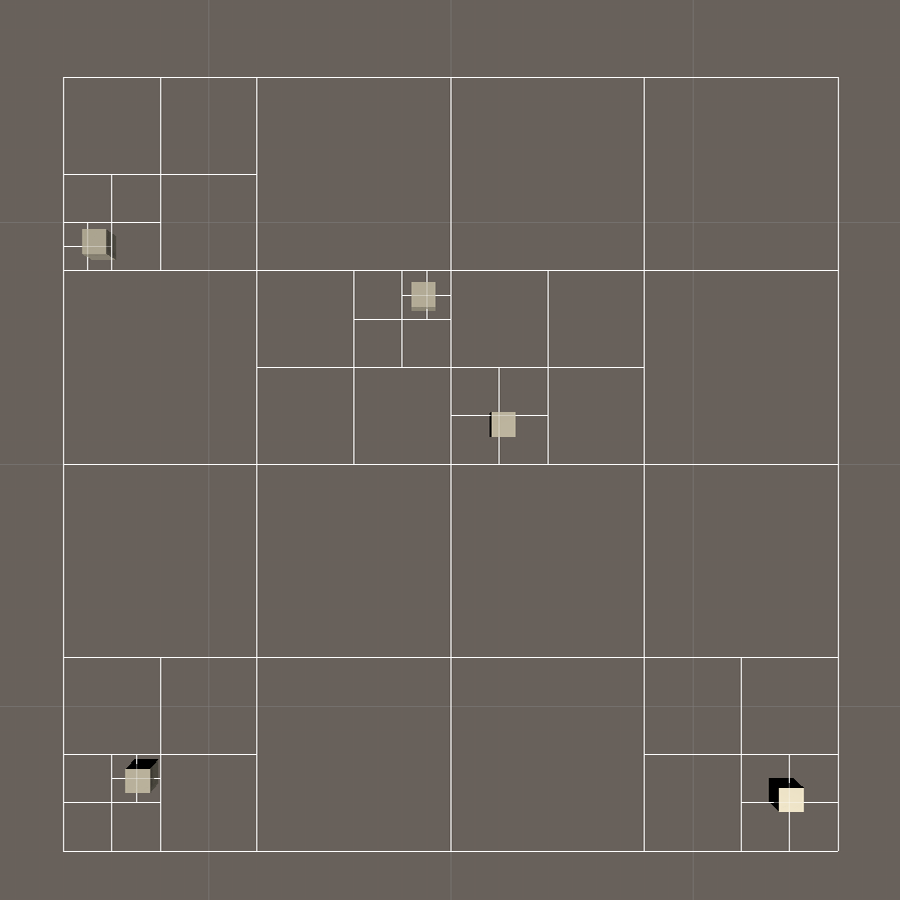
\includegraphics[width=.75\textwidth]{iso_top.png}
    \caption{Visualization of the quadtree structure for 5 \texttt{GameObject}s}
    \label{fig:demo:overview}
    \medskip\small
    A~view of the gizmos generated by the quadtree implementation for Unity's \texttt{GameObject}s from the editor.
\end{figure}

\section{Package Contents}
\begin{description}
    \item[\texttt{Scenes/}]
    directory contains example Unity scene(s) demonstrating usage of the package.
    
    \item[\texttt{Documentation/}]
    directory contains offline documentation.
    
    \item[\texttt{Scripts/}]
    directory contains all package's script source codes.
\end{description}

%-----------------------------------------------------------
%   Usage details
%-----------------------------------------------------------
\section{Usage} \label{usage}
This section describes the usage of the scripts provided by this package.
Simple editor usage for \texttt{GameObject}s with \texttt{Renderer} components is described in \ref{usage:editor}.
Section \ref{usage:code} then describes how to use the structures in the scripts.

\subsection{From Editor (Out of the Box)} \label{usage:editor}
Section \ref{usage:editor:store} explains how are objects stored in the tree structure and how it is set-up.
Then section \ref{usage:editor:find} gives an example how to search the structure and find previously stored objects.
Finally section \ref{usage:editor:remove} describes how the item removal from the tree works and is used.

\subsubsection{Setting Up the Tree} \label{usage:editor:setup}
Before we can play with the items in the tree, we first need to add a~root of our quadtree to the scene.
The initial setup of the root of the quadtree is extremely simple:
\begin{itemize}
    \item Create empty \texttt{GameObject}.
    
    This can be done by right-clicking in the \textit{Hierarchy} window and selecting \say{Create Empty}.
    \texttt{GameObject} you've now created will be used as a~root for the tree.
    Keep your newly created empty \texttt{GameObject} instance selected.
    
    \item From window dropdown menu select: \textit{Component > Spatial partitioning > Quadtree > Rootnode (for GameObjects)}.
    
    This command will add \texttt{GameObjectQuadtreeRoot} script component to the previously created \texttt{GameObject}.
    At this point you should be able to see white rectangle on the screen (make sure your gizmos are enabled and showing up in the editor).
\end{itemize}

\subsubsection{Storing Objects} \label{usage:editor:store}
Now with the tree root set-up 
\begin{itemize}
    \item Add \texttt{GameObject}s you wish to be in the tree as children of the tree root \texttt{GameObject}.
    
    The item must have any \texttt{Renderer} component\,---\,\texttt{MeshRenderer}, \texttt{SpriteRenderer}, \dots
    For example create any \texttt{GameObject} with \texttt{Renderer} component\,---\,do that by right-clicking on the tree root \texttt{GameObject} and selecting anything from submenu \textit{3D Object} or add your own!
    You've now added object supported by the quadtree, keep it selected in the \textit{hierarchy} window.
    
    \item From window dropdown menu select: \textit{Component > Spatial partitioning > Quadtree > Items > Renderer-based Item}.
    
    This command will add \texttt{RendererItem} script component to the previously added \texttt{GameObject}.
    At this point you should be able to see that the previous simple rectangle has somewhat changed.
    Try moving the item around, you should see the quadtree structure changing based on the current position of the item.
\end{itemize}

\subsubsection{Looking up Objects} \label{usage:editor:find}
Looking up objects from editor does not make much sense, since you will probably want to look the items up in a~code which will then work with them.
How to look up the objects in the tree is described in section \ref{usage:code:find}.

\subsubsection{Removing Objects} \label{usage:editor:remove}
Removing the items stored in the tree with \texttt{Renderer}-based item components is just removing either the \texttt{RendererItem} script component from the \texttt{GameObject} or removing the \texttt{GameObject} itself.
Simple as that.

\subsection{From Code} \label{usage:code}
This section describes how can you control the tree structure from the code.

\subsubsection{Storing Objects} \label{usage:code:store}
The stored items do not necessarily need to be children of the root node, but it allows the tree to fill completely automatically.
You can add items to the tree using scripts too, thought the item type must match with the item type of the tree root.
To add item to the tree follow the code shown in Listing \ref{code:insert}.

\begin{listing}[H]
    \begin{minted}{csharp}
// get the tree root component of the tree you want to insert to
var root = GetComponent<GameObjectQuadtreeRoot>();
// locate the GameObject to be added into the tree
var itemGO = GameObject.Find("Game Object Name");

// locate the tree item component of the GameObject
var item = itemGO.GetComponent<RendererItem>();

// insert the item to the tree using the Insert method
// the tree itself will find the smallest node to store it in
root.Insert(item);
    \end{minted}
    \vspace{-1em}
    \caption{Inserting Item to the Tree} \label{code:insert}
    \smallskip\small\centering
    This code snippet first locates the root of the quadtree, the \texttt{GameObject} to be inserted into the tree and its quadtree item component.
    Algorithm then inserts the item component into the tree via its root.
\end{listing}

\subsubsection{Looking up Objects} \label{usage:code:find}
To look up the stored objects you will need to use Unity's \texttt{Bounds}\footnote{\url{https://docs.unity3d.com/ScriptReference/Bounds-ctor.html}} object.
This object describes an area in which the algorithm will look for the items.
Follow code shown in Listing \ref{code:look_up}.

\begin{listing}[H]
    \begin{minted}{csharp}
// get the tree root component of the tree you want to search in
var root = GetComponent<GameObjectQuadtreeRoot>();

// locate or define the Bounds to be used in the search
// bounds defined below will find all items with bounds
// intersecting between (-5, 0, -5) and (5, 0, 5)
var bounds = new Bounds(Vector3.zero, new Vector3(10f, 0f, 10f));

// pass the bounds to the Find method of the root and
// the tree itself will find all the items with intersecting bounds
var items = root.Find(bounds);

// the Find method returns List of all found items
// continue as you will
foreach (var item in items)
{
    // process found items ...
}
    \end{minted}
    \vspace{-1em}
    \caption{Looking Up Stored Objects} \label{code:look_up}
    \smallskip\small\centering
    This code snippet first locates the root of the quadtree and creates the \texttt{Bounds} object which defines the search area.
    Algorithm then locates all items intersecting with the provided \texttt{Bounds} via tree root.
\end{listing}

% TODO: Create image visually depicting the search process and matching items

\subsubsection{Removing Objects} \label{usage:code:remove}
Removing the items from the tree is as easy as adding them in.
There are actually two ways to delete the item from the tree.
The location of the \texttt{GameObject} and its tree item component is the same for both possibilities.

The first removal option is to use the reference to the parent node, by which is the item currently contained, from the item object instance.
Since the item is actually contained by that node, the algorithm won't have to traverse the tree and look for the node which contains the item.
With the variables defined in the snippet above:

\begin{listing}[H]
    \begin{minted}{csharp}
// locate the GameObject to be removed from the tree
var itemGO = GameObject.Find("Game Object Name");
// locate the tree item component of the GameObject
var item = itemGO.GetComponent<RendererItem>();

// task the parent node with the removal of the item from the tree
item.ParentNode.Remove(item);
    \end{minted}
    \vspace{-1em}
    \caption{Removing the Item Via Its Parent Node} \label{code:remove:1}
    \smallskip\small\centering
    This code snippet removes the \texttt{GameObject}'s quadtree item from the tree via its own reference to the node in which it is currently contained.
\end{listing}

The second option is to pass the item to the tree root itself to remove the item.
The algorithm will have to traverse the tree to find correct node to remove the item from hence the former removal option is faster than the latter.
With the variables defined in the snippet above:

\begin{listing}[H]
    \begin{minted}{csharp}
// locate the GameObject to be removed from the tree
var itemGO = GameObject.Find("Game Object Name");
// locate the tree item component of the GameObject
var item = itemGO.GetComponent<RendererItem>();

// get the tree root component of the tree you want to remove from
var root = GetComponent<GameObjectQuadtreeRoot>();

// task the tree root with the removal of the item
root.Remove(item);
    \end{minted}
    \vspace{-1em}
    \caption{Removing the Item via Tree Root} \label{code:remove:2}
    \smallskip\small\centering
    This code snippet removes the \texttt{GameObject}'s quadtree item from the tree via root of the tree.
\end{listing}


%-----------------------------------------------------------
%   Implementation details
%-----------------------------------------------------------
\section{Implementation Details} \label{details}
This section aims to explain some important thoughts behind implementation of this library.
It should help you understand how is this library supposed to generally work.
The goal of this library is to allow maximum flexibility for you\,---\,the data structures are designed to allow \textit{any} items to be stored in the tree\,---\,the only requirement is implementation of predefined interface of the items.

As part of this package, there is already prepared tree item implementation supporting any \texttt{GameObject} instances with \texttt{Renderer} components.
This implementation works out of the box.

\subsection{Tree Root} \label{details:root}
Tree root represents the tree itself and provides an entry point for all the algorithms operating on the tree structure.
There always is only single tree root for a~single tree instance.
Tree root class is the main interface of the quadtree\,---\,any search, insertion or deletion starts in the root of the tree.

\begin{minted}{csharp}
public interface IQuadtreeRoot<TItem, TNode>
    where TItem : IItem<TItem, TNode>
    where TNode : INode<TItem, TNode>
\end{minted}

This is the interface that any tree root implementation should have.
Thought if you wish to implement your own tree root class from scratch nothing is stopping you!
Of course extending either \texttt{QuadtreeRoot} or \texttt{QuadtreeMonoRoot} is a~more sensible thing to do.
More on that topic in section \ref{extensions:custom_roots}.

\begin{minted}{csharp}
public class QuadtreeRoot<TItem, TNode> : IQuadtreeRoot<TItem, TNode>
    where TItem : IItem<TItem, TNode>
    where TNode : INode<TItem, TNode>, new()
\end{minted}

This is the actual used class implementing all that is necessary for a~tree root.
It allows anyone to further specify \texttt{TItem} and \texttt{TNode} which are classes of the items, respectively the nodes of the tree.
The only constraint for item classes is an implementation of interface \texttt{TItem}.
Tree node classes must implement \texttt{TNode} interface and have a parameterless constructor.

The previously mentioned class \texttt{QuadtreeMonoRoot} does actually not derive from \texttt{QuadtreeRoot}, because C\# does not allow multiple inheritance and to be able to use the class as a~\texttt{GameObject} component in Unity it must derive from \texttt{MonoBehaviour}.
Hence \texttt{QuadtreeMonoRoot} only implements the interface \texttt{IQuadtreeRoot} as a~proxy of \texttt{QuadtreeRoot}.
The class \texttt{GameObjectQuadtreeRoot} then derives from \texttt{QuadtreeMonoRoot} and specifies its type arguments as shown below.
Fully specifying types for generic classes is the last required step for the class to be used as a~\texttt{GameObject} component.

\begin{minted}{csharp}
public class GameObjectQuadtreeRoot : QuadtreeMonoRoot<GameObjectItem, Node<GameObjectItem>>
\end{minted}

\subsection{Tree Node} \label{details:node}
The \texttt{Node} class represents hierarchy of the tree.
It contains items stored in the tree and nodes which are lower in the hierarchy but still within its own boundaries.
There is usually no need to work with the nodes themselves\,---\,all actions should be done through root of the tree.
As mentioned before every node implementation must implement the \texttt{INode} interface.

\begin{minted}{csharp}
public interface INode<TItem, TNode>
    where TItem : IItem<TItem, TNode>
    where TNode : INode<TItem, TNode>
\end{minted}

If it does and also has a~public parameterless constructor, then you can use it instead of original \texttt{Node} implementation.
More about implementing custom node classes in section \ref{extensions:custom_nodes}.

The original implementation of the tree \texttt{Node}s derives from \texttt{NodeBase} which actually implements all the necessary functionality and, of course, the \texttt{INode} interface.
What \texttt{Node} does is just type specification of the \texttt{TNode} type parameter of the \texttt{NodeBase} class.

\begin{minted}{csharp}
public class Node<TItem> : NodeBase<TItem, Node<TItem>>
        where TItem : IItem<TItem, Node<TItem>> {}
\end{minted}

\subsection{Tree Item} \label{details:item}
Tree item classes represent the items in the tree.
All the classes must implement the \texttt{IItem} interface so the nodes know how to operate with the items.
More about implementing custom item classes in section \ref{extensions:custom_items}.

\begin{minted}{csharp}
public interface IItem<TItem, TNode>
    where TItem : IItem<TItem, TNode>
    where TNode : INode<TItem, TNode>
\end{minted}

The implementation for \texttt{GameObjects} uses a~number of classes but almost all the necessary logic is contained in the \texttt{GameObjectItemBase} class.
This class implements the \texttt{IItem} interface and all the necessarry logic for subclasses to work \textit{almost} automatically.
The \texttt{GameObjectItemBase} is implemented as \mintinline{csharp}{abstract} and requires only \texttt{GetBounds()} \textit{(and \texttt{This()})} method to be implemented by its subclasses.
It also derives from \texttt{MonoBehaviour} so it can be used as a~\texttt{GameObject} component.

\begin{minted}{csharp}
public abstract class GameObjectItemBase<TItem, TNode>
    : MonoBehaviour, IItem<TItem, TNode>
    where TItem : IItem<TItem, TNode>
    where TNode : INode<TItem, TNode>
\end{minted}

The \texttt{GameObjectItem} class then derives from \texttt{GameObjectItemBase}.
It, again, only specifies the type parameters of its superclass and extremely simple implementation of the \texttt{This()} method necessary for correct type checking.

\begin{minted}{csharp}
public abstract class GameObjectItem
    : GameObjectItemBase<GameObjectItem, Node<GameObjectItem>>
{
    protected override GameObjectItem This() => this;
}
\end{minted}

Finally the \texttt{RendererItem} class comes into light.
It further derives from \texttt{GameObjectItem} and implements the required \texttt{GetBounds()} method so the \texttt{GameObjectItemBase} can work properly.
This class specifically extracts the bounds from the \texttt{Renderer} component of the \texttt{GameObject} it is currently attached to.

%-----------------------------------------------------------
%   Extending implementation
%-----------------------------------------------------------
\section{Extending Implementation} \label{extensions}
Implementing custom structures and modifying existing ones should be pretty straightforward.
Just subclass the structure you wish to modify, override the implemented methods, et voilà!
It should be that simple.

\subsection{Custom Items} \label{extensions:custom_items}
If you implement custom item classes you will also need to create a~custom tree root implementation which supports usage of those items (exception to this are subclasses of \texttt{GameObjectItem} using \texttt{GameObjectQuadtreeRoot}).
But this is very simple too, as shown below.

\begin{minted}{csharp}
public class CustomItem : IItem<CustomItem, Node<CustomItem>>
{
    // TODO: Implement required interface of IItem here
}

public class CustomQuadtreeRoot : QuadtreeRoot<CustomItem, Node<CustomItem>> {}
\end{minted}

\subsection{Custom Nodes} \label{extensions:custom_nodes}
It's the same thing with the nodes as it is with the items\,---\,ff you implement custom node classes you will also need to create a~custom tree root implementation which supports usage of those items.

\begin{minted}{csharp}
public class CustomNode<TItem> : NodeBase<TItem, CustomNode<TItem>>
    where TItem : IItem<TItem, CustomNode<TItem>>
{
    // TODO: Override the NodeBase methods here
}

public class CustomQuadtreeRoot : QuadtreeRoot<CustomItem, CustomNode<CustomItem>> {}
\end{minted}

\subsection{Custom Roots} \label{extensions:custom_roots}
As shown a~number of times in the previous sections\,--\,creating a~custom tree root implementation is quite simple.
No class body has been provided in the previous section since modification of the item's or node's type has been enough, but you can override any method of your choosing of course.

\begin{minted}{csharp}
public class CustomQuadtreeRoot : QuadtreeRoot<CustomItem, CustomNode<CustomItem>>
{
    // TODO: Override the QuadtreeRoot methods here
    // TODO: Implement custom methods here
}
\end{minted}

\end{document}
